\documentclass[11pt,a4paper,oneside]{book}

\setlength{\parindent}{0cm}

\usepackage{color}
\usepackage{graphicx}
\usepackage{hyperref, url}
\usepackage{listings}

\usepackage{gmutils}
\usepackage{makeidx}
\makeindex

\begin{document}

\newcommand{\tableheader}[1]{\textbf{#1}}
\newcommand{\ientry}[1]{#1\index{#1}}
\newcommand{\imentry}[1]{#1\index{#1|\textbf}}

\frontmatter
\title{Essential \LaTeXe{}}
\author{G.J.\ Bex (\url{geertjan.bex@uhasselt.be})}
\date{\today}

\maketitle
\tableofcontents

\mainmatter

\chapter{Introduction}
\label{ch:intro}

\section{What is \LaTeXe{}?}
\label{sec:what-is-latex}

\LaTeXe{} is a sophisticated typesetting system that was especially designed to produce beautiful material containing a lot of mathematical notation.  It will produce publication quality Postscript or PDF files as output.
\LaTeXe{} has been nearly universally  adopted among mathematicians, (theoretical) physicists, and computer scientists.  The original \TeX{} typesetting system from which \LaTeX{} and \LaTeXe{} can be considered descendants was developed by Donald E.\ Knuth, while the  original \LaTeX{} was created by Leslie Lamport.  Currently, only the modern form, \LaTeXe{}, should be used.

The biggest selling point of \LaTeXe{} with respect to other document processing tools such as Microsoft Word is that markup is primarily semantic in nature, i.e., the markup conveys meaning, rather than style information.  This implies that the same \LaTeXe{} source can be typeset in many different styles by changing the mapping from semantics to layout.
An example of this is the \verb|\emph{here}| command that implies that its argument is emphasized.  Contrast this to \verb|\textit{here}| which indicates that the text should be set in italics.  The visual result is the same, as illustrated \emph{here}, versus \textit{here}, but it should be clear that the former is much more informative to the authors.


\section{Scope of this Document}
\label{sec:scope}

This text is intended for those who write manuals, or tutorial information related to software and computational services.  As such, it discusses only issues that are useful in that context.  One area which is not covered at all, although it is where \LaTeXe{} truly excels is typesetting mathematical formulas.

Although many GUI programs exist to edit and typeset \LaTeXe{} documents, this text will be restricted to command line tools only.  High-quality distributions are available for all major platforms.

To typeset a document, e.g., for the file \verb|latex-intro.tex|, simply use the following command line commands in your favorite shell and terminal:
\begin{verbatim}
    $ pdflatex latex-intro
\end{verbatim}
Note that typically two passes may be needed in order to get references right.  This will produce a number of artifacts: \verb|latex-intro.aux|, \verb|latex-intro.log|, and most importantly, \verb|latex-intro.pdf|.

For documents that include a bibliography (see Section~\ref{sec:bibliography}) or an index (see Section~\ref{sec:index}), one should consider using the GNU make tool for streamlining the typesetting process.

Currently, defining one's own command and environments is beyond the scope of this introduction, although the document contains a few examples for the curious reader.  More information on this topic, and on anything else missing from this text can be found in the excellent guide to \LaTeX{ by Kopka and Daly~\cite{Kopk04}.


\section{Some advice}
\label{sec:advice}

As mentioned before, \LaTeXe{} offers much potential to produce exquisite looking documents.  All and every aspect can be fine tuned for optimal results.  Just as with code development however, it is best to resist the urge to embark on micro optimization.  Postpone fine tuning the appearance of a document until the contents is at least mostly stable.  The appearance of a document is very brittle, so minor additions or deletions may have a major impact on, e.g., page layout.

However, if one is working on a new document, it may be wise to keep features like an index or a glossary in mind when starting to write, because adding those later when the text is finished is going to be more labor intensive.

The major point however, is to concentrate on content and its semantics, and keep this firmly separated from layout and appearance.


\chapter{Document Structure}
\label{ch:doc-struct}

A typical \LaTeXe{} document consists of a number of parts that will be discussed one by one in this chapter.  To help the reader, a skeleton document has been created in Listing~\ref{lst:latex-skel}.

\section{Document classes}
\label{sec:doc-classes}

Each \LaTeXe{} document is an instance of a class, most relevant are \verb|article|, \verb|report|, and \verb|book|.  The declaration of the \ientry{document class} specifies some formatting information, e.g.,
\begin{verbatim}
  \documentclass[11pt,a4paper,oneside]{book}
\end{verbatim}
Here, the default font size is set to 11 point, the paper format to A4, while we specify that the book should be typeset for printing one sided.

\section{Packages}
\label{sec:packages}

A very nice feature of \LaTeXe{} is that a large number of extension packages are available.  Many have been designed to facilitate producing beautiful material for specific scientific disciplines, such as Feynman diagrams in quantum mechanics.  Others are more generally applicable such as \verb|hyperref| that will automatically introduce links in PDF documents, or \verb|url| that can be used to typeset web links or email addresses.  These packages often interact, e.g., when using both \verb|hyperref| and \verb|url|, web links and email addresses are hyperlinked as well.

Packages can be included easily:
\begin{verbatim}
    \usepackage{hyperref, url}
\end{verbatim}

Some packages can be configured by specifying options when importing them, e.g.,
\begin{verbatim}
    \usepackage[english]{babel}
\end{verbatim}
The \verb|babel| package takes care of such things as correct hyphenation for a language (\emph{non-trivial}), and is extremely useful when authoring multi-lingual documents.  Here, it is specified that this document will use only English.

Although most modern \LaTeXe{} distributions come with a plethora of packages, it is useful to check out CTAN (\url{http://www.ctan.org}).

\section{Book structure}
\label{sec:book-struct}

The actual contents of the book is in the \verb|document| environment, i.e.,
\begin{verbatim}
    \begin{document}

    \end{document}
\end{verbatim}
A book consists of three parts:
\begin{enumerate}
    \item \verb|\frontmatter|, see Section~\ref{sec:front-matter}
    \item \verb|\mainmatter|, see Section~\ref{sec:main-matter}
    \item \verb|\backmatter|, see Chapter~\ref{ch:icing}
\end{enumerate}
The \ientry{front matter} is intended for the book's title page, its table of contents, and such.  The \ientry{main matter} contains the actual chapters, and, optionally appendices.  The \ientry{back matter} is intended for the index, a glossary, the bibliography, \ldots

\subsection{Front matter}
\label{sec:front-matter}

One of the things \LaTeXe{} can do automatically, is create a title page.  It is a simple matter to specify some meta information, e.g.,
\begin{verbatim}
    \title{A Short Guide to \LaTeXe{}}
    \author{G.J.\ Bex (\url{geertjan.bex@uhasselt.be})}
    \date{\today}
\end{verbatim}
Note the use of the \verb|\url{}| command for the author's email address.

A title page, as well as the table of contents is now automatically generated by:
\begin{verbatim}
    \frontmatter
    \maketitle
    \tableofcontents
\end{verbatim}
Thanks to using the \verb|hyperref| package, the table of contents will contain hyperlinks to its entries.

If the auto-generated title page is not to one's liking, it is easy to create one as sophisticated as one likes using the \verb|titlepage| environment.

\subsection{Main matter}
\label{sec:main-matter}

As mentioned before, the main matter contains the actual book chapters.  Optionally, a book can have multiple parts as well.  To begin a new chapter, simply use:
\begin{verbatim}
    \chapter{What is \LaTeXe{}?}
    \label{ch:what-is-latex}
\end{verbatim}
Basically, one states the chapter's title, and specifies a label that can be used to refer to it later.  A chapter ends when the next chapter begins, or when the back matter starts.

A chapter typically consists of multiple sections, that can each have subsections.  Sections are started similarly to chapters, e.g.,
\begin{verbatim}
    \section{Document classes}
    \label{sec:document-classes}
\end{verbatim}
A section ends at the start of the next, or when a new chapter begins.

The contents hierarchy for a book is:
\begin{itemize}
    \item \verb|\part|
    \item \verb|\chapter|, \verb|\appendix|
    \item \verb|\section|
    \item \verb|\subsection|
    \item \verb|\subsubsection|
\end{itemize}
Note that all these structural parts of a document are automatically added to the table of contents.  Also note that it is good practice to use a prefix for labels in order to more easily tell them apart, e.g., \verb|ch:| for chapters, \verb|sec:| for sections.


\chapter{Formatting Text}
\label{ch:formatting-text}

\section{Text and special characters}
\label{sec:text-specials}

Typically, \LaTeXe{} source code for ordinary text is just that, i.e., ordinary text.  There are a few things to keep in mind though.  Since \LaTeXe{} is a programming language of sorts, certain characters are part of that language, and have to be escaped.  The following is a list of such \ientry{command characters}.
\begin{itemize}
    \item \# $=$ \verb|\#|
    \item \$ $=$ \verb|\$|
    \item \& $=$ \verb|\&|
    \item \_ $=$ \verb|\_|
    \item \% $=$ \verb|\%|
    \item \{ $=$ \verb|\{|
    \item \} $=$ \verb|\}|
\end{itemize}
\LaTeXe{} also comes with support for \ientry{diacritical characters} that is sufficient for most Latin based European scripts.  A few examples that are useful for French, German, and Dutch:
\begin{itemize}
    \item \'{e} $=$ \verb|\'{e}|
    \item \`{e} $=$ \verb|\`{e}|
    \item \^{e} $=$ \verb|\^{e}|
    \item \"{o} $=$ \verb|\"{o}|
    \item {\ss} $=$ \verb|{\ss}|
    \item \"{\i} $=$ \verb|\"{\i}|
\end{itemize}
In nicely typeset text, three types of hyphens and dashes are used, compare opt-in (\ientry{hyphen}), with 5--10 (\ientry{en-dash}), and the one that---although rarely used---nevertheless (\ientry{em-dash}) deserves to look beautiful.  They have been produced with \verb|-|, \verb|--|, and \verb|---| respectively.

\ientry{Quotation marks} also deserve a little attention, since the starting quotation mark is typeset with a character that is distinct from the end quotation mark.  The `single quotes' and ``double quotes'' in this sentence were produced using \verb|`single quotes'| and \verb|``double quotes''| respectively.

To start a new \ientry{paragraph}, an empty line is inserted between blocks of text.  For the default style, the first paragraph of a chapter or a section is not indented, subsequent paragraphs are.  This may or may not be to one's liking, and can be controlled by setting the value of \verb|\parindent| to $0 \mathrm{cm}$, as was done for this document.  Manuals often tend to have many short paragraphs, and the author thinks the paragraph indentation is ugly in that case, but feel free to disagree.

To start a new line without starting a new paragraph, one simply ends the line with \verb|\\|.  This can often be very useful in special cases such as formatting tables, but should be used sparingly in running text.

\section{Fonts\ldots or not}
\label{sec:fonts}

\LaTeXe{} allows the author to explicitly change the format of text by specifying attributes such as font size, of face.  For example, the following code fragment would produce the paragraph below it.
\begin{verbatim}
    The following word is {\Large large}, while the next is
    \textbf{bold}, and this one is in \textit{italics}.  
\end{verbatim}
\begin{quote}
    The following word is {\Large large}, while the next is \textbf{bold}, and this one is in \textit{italics}.  
\end{quote}
However, this approach is rarely good practice.  Typically, font attributes are intended to convey meaning, e.g., text may be set in italics to emphasize it.  Hence, it is better style to use the appropriate commands that are defined for precisely that purpose, e.g., \verb|\emph{emphasize}| will produce \emph{emphasize}, and indicate the author's intent.  If you feel tempted to use explicit formatting commands, think again, it is probably not what you \emph{really} want.


\section{Lists}
\label{sec:lists}

Although lists are extremely customizable in \LaTeXe{}, three predefined types are definitely most useful: \verb|itemize|, \verb|enumerate|, and \verb|description|, each implemented as an environment.
Lists can be nested to create multi-level lists, e.g.,
\begin{verbatim}
    \begin{enumerate}
        \item Lists are nice.
        \item Lists can be nested, i.e.,
            \begin{enumerate}
                \item each item can start a new environment, and
                \item they can, but need not be the same type.
            \end{enumerate}
    \end{enumerate}
\end{verbatim}
This code fragment produces the following text.
\begin{enumerate}
    \item Lists are nice.
    \item Lists can be nested, i.e.,
        \begin{enumerate}
            \item each item can start a new environment, and
            \item they can, but need not be the same type.
        \end{enumerate}
\end{enumerate}

A descriptive list can be used to define a number of terms, e.g.,
\begin{description}
    \item[itemize] An environment to produce a bulleted list.
    \item[enumerate] An environment to produce a numbered list.
    \item[description] An environment to produce this list.
\end{description}


\section{Literal text and source code}
\label{sec:source-code}

This \LaTeXe{} source in this text has been typeset using the standard command \verb=\verb|\textit{here}|= and environment \verb|verbatim|.  Although this is sufficient to include some \LaTeXe{}, it falls short when one has to deal with source code for various programming languages, especially when such features as syntax highlighting are desired.

The package of choice for this purpose is \verb|listings|\footnote{\url{http://www.ctan.org/pkg/listings}}.  Out of the box it supports many programming languages, \verb|bash|, \verb|C|, \verb|Fortran|, \verb|Python|, and \verb|TeX| to name just a few.  For many languages, several dialects are supported, e.g., \verb|LaTeX| for \verb|TeX|.  It comes with a 50 pages+ manual, including sections on how to define support for your very own programming language.  To use \verb|listings| include in it the document's preamble, i.e.,
\begin{verbatim}
    \usepackage{listings}
\end{verbatim}
The canonical Hello World in C would be given by:
\begin{verbatim}
    \begin{lstlisting}[language=C,numbers=left,%
                       numberstyle=\tiny]
        #include <stdio.h>

        int main(int argc, char *argv[) {
            printf("hello world!\n");
            return 0;
        }
    \end{lstlisting}
\end{verbatim}
which produces:
\begin{lstlisting}[language=C,numbers=left, %
                   numberstyle=\tiny]
    #include <stdio.h>

    int main(int argc, char *argv[) {
        printf("hello world!\n");
        return 0;
    }
\end{lstlisting}

\lstset{language=C}
Inlining source code snippets is very similar to using \verb=\verb|\textit{here}|=, but it will respect the programming language syntax, e.g., assignments in declarations are as easy as \lstinline|const int n = 10;|.
It is also possible to include a standalone source file, as was done to produce Listing~\ref{lst:latex-skel}.  Although it is possible to use only parts of source code listings as input, this is usually not the best idea since it is very brittle, and creates a maintenance nightmare in the blink of an eye.  The following code fragment illustrates the input of external source code.
\begin{verbatim}
    \lstset{language=[LaTeX]TeX}
    \lstinputlisting[frame=single, float,  %
                     label=lst:latex-skel, %
                     caption=a \LaTeXe{} skeleton file]
                    {latex-skel.tex}
\end{verbatim}
Note the use of the label, similar to \verb|chapter| and \verb|section| to ensure that it will be possible to refer to this listing later.

\lstset{language=[LaTeX]TeX}
\lstinputlisting[frame=single, float,  %
                 label=lst:latex-skel, %
                 caption=a \LaTeXe{} skeleton file]
                {latex-skel.tex}

It should be clear that for any document that contains more than the odd listing, creating new environments to set a number of specific options may be a wise move.

\section{References}
\label{sec:references}

Labels have been introduced in Sections~\ref{sec:main-matter} and~\ref{sec:source-code} to facilitate referring to them in other parts of the text.  The references used here have been produced by the following code fragment:
\begin{verbatim}
    in Sections~\ref{sec:main-matter}
    and~\ref{sec:source-code} to
\end{verbatim}
Note that using references is one of the reasons it is typically necessary to typeset a document multiple times.  When labels are changed or added, an index is build during the first pass, and that information can only be used to show correct references upon the second pass.


\section{Tables}
\label{sec;tables}

Any half decent book on \LaTeXe{} has a full fledged chapter on tables.  Indeed, it is an extensive subject with many interesting aspects.  This Section will limit itself to the basics.  Creating a table is most easily done using the \verb|tabular| environment.
\begin{center}
    \begin{tabular}{|l|l|} \hline
        \tableheader{Site}      & \tableheader{Clusters} \\ \hline
        Antwerpen               & Turing, Hopper \\
        Brussels                & Hydra \\
        Gent                    & too many Pokemons to list \\
        Leuven                  & VIC3, ThinKing \\ \hline
    \end{tabular}
\end{center}
The table above was typeset using the following \LaTeXe{} fragment:
\begin{verbatim}
    \begin{tabular}{|l|l|} \hline
        \tableheader{Site}      & \tableheader{Clusters} \\ \hline
        Antwerpen               & Turing, Hopper \\
        Brussels                & Hydra \\
        Gent                    & too many Pokemons to list \\
        Leuven                  & VIC3, ThinKing \\ \hline
    \end{tabular}
\end{verbatim}
The positions specified as an option to the tabular environment specify the alignment, one for each of the table's columns.  These alignments can take the values \verb|l|, \verb|c|, and \verb|r| for left, centered, and right alignment respectively.  The vertical bar character \verb=|= is used to indicate that a vertical line should be drawn at that position in the table to separate columns.  To separate rows, the \verb|\hline| command can be used.

\section{Including figures}
\label{sec:figures}

\LaTeXe{} supports quite a number of formats to be included in documents, depending of the flavor of the typesetter used.  For \verb|pdflatex|, one can use PDF as vector format, and PNG for pixel based graphics, such as screenshots.  First of all, one has to include a package for using graphics, e.g., \verb|graphicx|.  After that, including a graphics file is as easy as using the following command:
\begin{verbatim}
    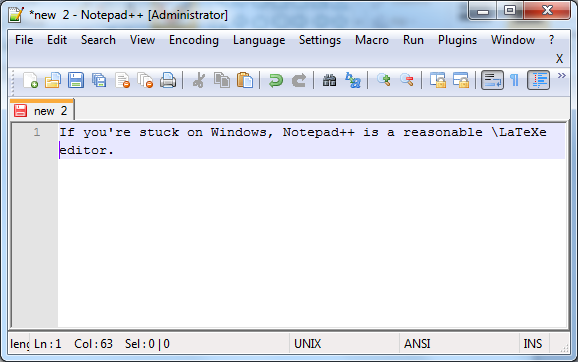
\includegraphics[width=10cm]{screenshot.png}
\end{verbatim}
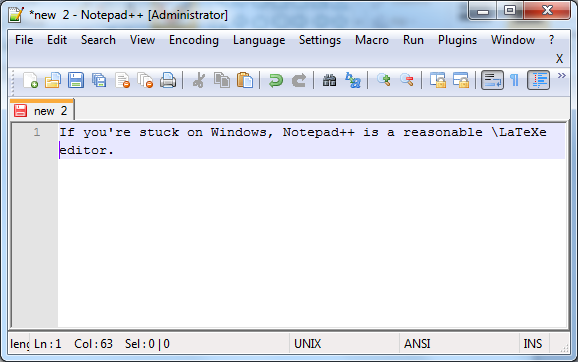
\includegraphics[width=10cm]{screenshot.png} \\
When only the width or height of a figure is specified, the figure will be scaled to that value, preserving the aspect ratio.

Typically, figures, and for that matter tables as well, are often included as floating elements.  For the figure above, that would be:
\begin{verbatim}
    \begin{figure}[h]
        \caption{\label{fig:notepad} Notepad++ is a Windows text editor}
        \begin{center}
            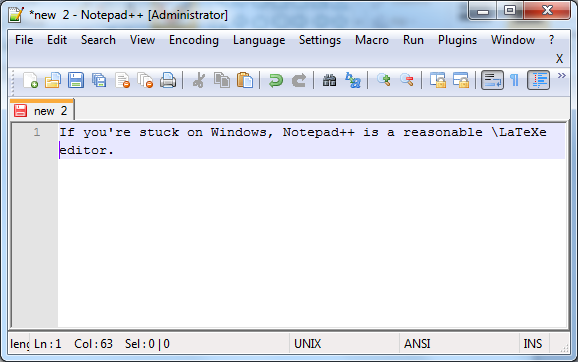
\includegraphics[width=10cm]{screenshot.png}
        \end{center}
    \end{figure}
\end{verbatim}

\begin{figure}[h]
    \caption{\label{fig:notepad} Notepad++ is a Windows text editor}
    \begin{center}
        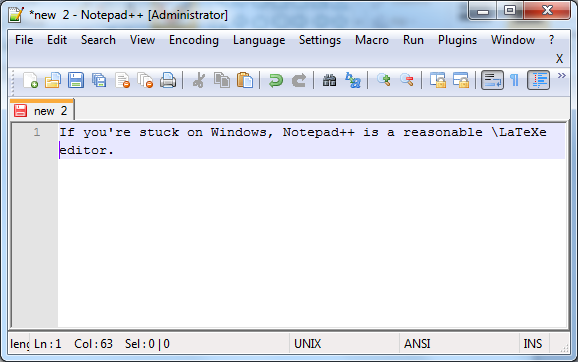
\includegraphics[width=10cm]{screenshot.png}
    \end{center}
\end{figure}

Note that Figure~\ref{fig:notepad} has a caption, and can be referred to, thanks to its label.  The placement of floating elements is done according to a number of rules that try to produce the best-looking output, and is better left to \LaTeXe{}.  One can give hints by specifying \verb|h| for ``here'', \verb|b| for ``bottom'', \verb|t| for ``top''.  Adding \verb|!| to that position hint makes the typesetter try harder to place the floating element were you indicate.

As mentioned before, tables can also be included as floating elements by embedding a \verb|tabular| environment into a \verb|table| environment, so that one can add a caption and label to refer to it.  The following code fragment produces Table~\ref{tbl:clusters}.
\begin{verbatim}
\begin{table}[h]
  \caption{\label{tbl:clusters} Clusters on various sites}
  \begin{tabular}{|l|l|} \hline
    \tableheader{Site}      & \tableheader{Clusters} \\ \hline
    Antwerpen               & Turing, Hopper \\
    Brussels                & Hydra \\
    Gent                    & too many Pokemons to list \\
    Leuven                  & VIC3, ThinKing \\ \hline
  \end{tabular}
\end{table}
\end{verbatim}

\begin{table}[h]
    \caption{\label{tbl:clusters} Clusters on various sites}
    \begin{center}
        \begin{tabular}{|l|l|} \hline
            \tableheader{Site}      & \tableheader{Clusters} \\ \hline
            Antwerpen               & Turing, Hopper \\
            Brussels                & Hydra \\
            Gent                    & too many Pokemons to list \\
            Leuven                  & VIC3, ThinKing \\ \hline
        \end{tabular}
    \end{center}
\end{table}

\chapter{Icing on the Cake}
\label{ch:icing}

\section{Creating a bibliography}
\label{sec:bibliography}

Many document---if not all in a scientific context---refer to books or articles, books, and other reference material.  Citing these references is very easy, e.g., this text could not have been written without consulting Kopka's excellent book~\cite{Kopk04}.  The citation is accomplished as follows:
\begin{verbatim}
    excellent book~\cite{Kopk04}.
\end{verbatim}

A separate file in \ientry{\BibTeX} format contains the actual bibliographic information and can be used to typeset any number of documents.  The entry cited here is shown in Listing~\ref{lst:bibtex}.

\lstinputlisting[caption=A very short \BibTeX file,label=lst:bibtex,
                 float,language=TeX]{vsc-refs.bib}

Obviously, such a file can be produced by hand, but there are a number of applications that really have added value when managing bibliographies, JabRef in particular\footnote{\url{http://jabref.sourceforge.net/}}.

Producing the bibliography requires an up-to-date \verb|.aux| file, and running the \verb|bibtex| command line tool that comes with the \LaTeX{} distribution.  This will produce a \verb|.bbl| file that is included automatically in the back matter by the following code fragment:
\begin{verbatim}
    \bibliography{vsc-refs} \bibliographystyle{alpha}
\end{verbatim}
Note that the \verb|bibliography| command specifies the \BibTeX file to use.

To actually create the bibliographic entries for later inclusion in the document, one has to run the \verb|bibtex| command line tool, e.g.,
\begin{verbatim}
    $ bibtex latex-intro
\end{verbatim}
Note that it takes another typesetting pass to include the bibliographic entries.


\section{Creating an index}
\label{sec:index}

Although the technical part of creating an index to a document is very simple, it is nevertheless very labor intensive since each entry has to be added by hand.  One has to indicate in the document's preamble that an index has to be created by loading the \verb|makeidx| package, and subsequently adding the \verb|\makeindex| command.  The index can be shown---typically in the back matter---by using the \verb|\printindex| command.

The next step is to mark the words that should go into the index using the \verb|\index{term}|, which would mark the word term for inclusion in the index at that position in the text.  As for creating bibliographies, one needs a command line tool to create an index.
\begin{verbatim}
    $ makeindex latex-intro
\end{verbatim}
Note that to include generated indices correctly, it takes a few typesetting passes.


\section{Creating a glossary}
\label{sec:glossary}




\backmatter

\bibliography{vsc-refs} \bibliographystyle{alpha}

\printindex

\end{document}

